\documentclass[conference]{IEEEtran}
\IEEEoverridecommandlockouts
% The preceding line is only needed to identify funding in the first footnote. If that is unneeded, please comment it out.
\usepackage{cite}
\usepackage{amsmath,amssymb,amsfonts}
\usepackage{algorithmic}
\usepackage{graphicx}
\graphicspath{{../part1/figures/}}
\usepackage{textcomp}
\usepackage{xcolor}
\def\BibTeX{{\rm B\kern-.05em{\sc i\kern-.025em b}\kern-.08em
    T\kern-.1667em\lower.7ex\hbox{E}\kern-.125emX}}
\begin{document}

\title{Evaluating Policy Gradient Methods and Domain Randomization for Sim-to-Real Robot Control\\
}

\author{\IEEEauthorblockN{Giuseppe Colazzo}
\IEEEauthorblockA{\textit{Master's Degree in Data Science and Engineering} \\
\textit{Politecnico of Turin}\\
Turin, Italy \\
s360736@studenti.polito.it}
\and
\IEEEauthorblockN{Francesco Federico}
\IEEEauthorblockA{\textit{Master's Degree in Data Science and Engineering} \\
\textit{Politecnico of Turin}\\
Turin, Italy \\
s355100@studenti.polito.it}
\and
\IEEEauthorblockN{Marco Macrì}
\IEEEauthorblockA{\textit{Master's Degree in Data Science and Engineering} \\
\textit{Politecnico of Turin}\\
Turin, Italy \\
s349228@studenti.polito.it}
\and
\IEEEauthorblockN{Filippo Montecchi}
\IEEEauthorblockA{\textit{Master's Degree in Data Science and Engineering} \\
\textit{Politecnico of Turin}\\
Turin, Italy \\
s361316@studenti.polito.it}
}

\maketitle

\begin{abstract}
This project investigates reinforcement learning for continuous robotic 
control and sim-to-real transfer in a sim-to-sim setting. The work is 
divided into two complementary parts: in the first, policy-gradient methods 
including REINFORCE, REINFORCE with baseline, and Actor-Critic are implemented 
and evaluated on the Hopper continuous-control environment, with improvements 
including Generalized Advantage Estimation, advantage normalization, a learned 
exploration variance with a sigma floor, and a triggered learning-rate decay 
mechanism; the resulting Actor-Critic agent achieved average rewards around 
2000 and individual episodes exceeding 3000, while the baseline variant reached 
a peak test reward of 2444 compared to 1305 for vanilla REINFORCE. In the 
second part, sim-to-sim transfer is investigated on the PandaPush environment 
using PPO, SAC, UDR, and ADR: SAC outperformed PPO, and UDR achieved the best 
transfer performance, reducing the sim-to-real gap by approximately 66\% 
relative to vanilla SAC. These results confirm the effectiveness of modern 
actor-critic methods for continuous control and show that domain randomization 
can substantially improve robustness under dynamics uncertainty.
\end{abstract}

\section{Introduction}
Reinforcement Learning has recently shown remarkable success in solving continuous control tasks, enabling agents to acquire manipulation and locomotion skills.

However, training these policies on real physical hardware is often unfeasible due to costs, mechanical wear and safety constraints.
As a result of this, the standard procedure relies on training these agents in simulated environments before deploying them into the real world.

A major challenge in this procedure is the \textit{reality gap}, the discrepancy between the simulated training environment and the actual world. This is often caused by unmodeled dynamics or sensor noise leading to a degradation of performance when moving from the simulation to the real world. 

The first part of this work focuses on the \texttt{Hopper-v4} locomotion task, an environment where a one-legged robot must learn to jump forward without falling. Within this setting, we implement the vanilla REINFORCE algorithm from scratch and evaluate the critical role of baseline subtraction by testing both a zero baseline and a constant baseline. 

Finally, we design and implement a one-step Actor-Critic architecture to show how bootstrapping and temporal difference learning can reduce gradient variance. This improves learning stability and speeds up policy convergence.


[[AGGIUNGERE QUI PARTE DUE SU PPO E SAC]]


\section{Methodology}
\subsection{Part 1: Hopper Continuous Control}

Idea:
\begin{itemize}
    \item Cite all methods used: REINFORCE with and without baseline + AC + GAE
    \item Briefly explain all methods added: GAE, normalised advantages, sigma floor, LR decay
    \item Should I use some references here for GAE, reinforce and actor critic?
\end{itemize}

Part 1 focused on learning a locomotion policy for the Hopper environment using policy-gradient methods. Several approaches were explored, including REINFORCE, REINFORCE with baseline, and Actor-Critic architectures \cite{sutton2018}.

Since we're considering a continuous enviroment, all models policy outputs both the mean and standard deviations of a Gaussian action distribution, $a_t \sim \mathcal N(\mu_\theta(s_t), \sigma_\theta(s_t))$, where both parameters are learned by the policy network. During training, actions are sampled from the distribution to encourage exploration, while during evaluation the policy becomes deterministic by using mean actions $\mu_\theta(s_t)$.

To improve the quality of the policy updates, Generalized Advantage Estimation (GAE) was implemented \cite{schulman2015}. Therefore, advantages are computed as
\[
\hat A_t^{GAE} = \sum_{l=0}^{\infty} (\gamma\lambda)^l \delta_{t+l}
\]
Where $\delta_t = r_t + \gamma V(s_{t+1}) - V(s_t)$ is the temporal-difference error.
In this way, GAE provides a compromise between using a low-variance TD(0) estimate and a high variance Monte Carlo approach that considers the episode full return.

Subsequently, advantages were normalized before policy updates in order to stabilize gradients, stabilize critic's estimates and reduce training instability. A minimum standard deviation (sigma floor) was enforced to prevent premature collapse of exploration and continue promoting exploration even in later stages. Additionally, a triggered learning-rate decay mechanism was introduced during later stages of training with the aim of stabilizing training by reducing update magnitude after the policy had discovered effective locomotion behaviors.

All these modifications were designed to improve training stability, maintain sufficient exploration, and allow longer training horizons without facing policy collapses.


\subsection{Part 2: PandaPush, SAC, PPO and Domain Randomization}

Idea:
\begin{itemize}
    \item Not sure about anything I'm saying, check pls + it's pretty AI
\end{itemize}

Part 2 investigates sim-to-real transfer using the PandaPush-v3 robotic manipulation environment. The task consists of controlling a Franka Panda robotic arm to push a cube toward a desired target position.
The observation space contains the robot state, cube state, and target position information. Actions are continuous Cartesian end-effector displacements,
\[
a_t=[dx,dy,dz].
\]
The dense reward function is defined as
\[
r_t = -\left\| p_{obj}(t)-p_{goal} \right\|_2,
\]
where $p_{obj}$ and $p_{goal}$ denote the cube and target positions respectively. A task is considered successful when the final cube-target distance is below 5 cm.

Two reinforcement-learning algorithms were evaluated.
Proximal Policy Optimization (PPO) is an on-policy actor-critic algorithm that limits policy updates through a clipped objective,
\[
L^{CLIP} = \mathbb E \Big[ \min( \rho_t \hat A_t, \text{clip}(\rho_t,1-\epsilon,1+\epsilon)\hat A_t ) \Big].
\]
The clipping mechanism improves stability but reduces sample efficiency because collected trajectories cannot be reused extensively.

Soft Actor-Critic (SAC) is an off-policy actor-critic method that maximizes both reward and policy entropy,
\[
J = \mathbb E[R] + \alpha H(\pi).
\]
SAC combines a replay buffer, twin critics to reduce value overestimation, and automatic entropy tuning. These characteristics generally provide better exploration and sample efficiency than PPO, especially in continuous-control robotic tasks.
To improve transfer across different dynamics, Domain Randomization (DR) was applied by varying the cube mass during training.

Three configurations were evaluated:
\begin{itemize}
    \item No DR: fixed source mass $m=1$ kg.
    \item Uniform Domain Randomization (UDR): $m \sim U(0.5,8.0)$ with a new mass sampled at every episode.
    \item Automatic Domain Randomization (ADR): an adaptive curriculum that expands or contracts the sampling range according to agent performance.
\end{itemize}

The target environment uses a cube mass of 5 kg. However, the randomization range was chosen to be broad enough to include both source and target conditions without being narrowly centered around the target mass, avoiding information leakage from the evaluation environment.



\section{Experiments \& Results}

\subsection{Part 1 Results: Hopper Continuous Control}

All three algorithms were trained for 70{,}000 episodes on the Hopper-v4 environment, repeated across three independent seeds.
Table~\ref{tab:part1_results} summarises the training performance;
Figure~\ref{fig:experiments_reward} shows the learning curves (rolling average over 100 episodes $\pm$ standard deviation across seeds).

In the table, \emph{Best Avg-100} is the peak value of the 100-episode rolling mean (averaged over seeds);
\emph{Final Avg-100} is the mean return over the last 100 training episodes; \emph{Std} is the standard deviation computed over all 70{,}000 episodes across all seeds;
\emph{Best Episode} is the highest single-episode return observed per seed, averaged across seeds;
\emph{Avg Ep.\ Len} is the mean episode length over the full 70{,}000 training episodes across all seeds;
\emph{Time (min)} is the total time required to train the agent.



\begin{table}[ht]
\centering
\caption{training performance on Hopper-v4 (mean over 3 seeds).}
\label{tab:part1_results}
\resizebox{\linewidth}{!}{%
\renewcommand{\arraystretch}{1.2}
\begin{tabular}{lrrrrcc}
\hline
\textbf{Algorithm} & \textbf{Best Avg-100} & \textbf{Final Avg-100} & \textbf{Std} & \textbf{Best Episode} & \textbf{Avg Ep.\ Len} & \textbf{Time (min)} \\
\hline
REINFORCE ($b{=}0$)  & 1006 & 635  & 257 & 2811 & 178 & 57.6 \\
REINFORCE ($b{=}20$) & 1807 & 806  & 399 & 3152 & 215 & 70.3 \\
Actor-Critic         & \textbf{1938} & \textbf{1360} & \textbf{734} & \textbf{3480} & \textbf{249} & \textbf{83.8} \\
\hline
\end{tabular}%
}
\end{table}

\begin{table}[ht]
\centering
\caption{test performance on Hopper-v4.}
\label{tab:part1_test_results}
\resizebox{\linewidth}{!}{%
\renewcommand{\arraystretch}{1.2}
\begin{tabular}{lccc}
\hline
\textbf{Algorithm} & \textbf{Seed} & \textbf{Test Return (Mean $\pm$ Std)} & \textbf{Test Length (Mean $\pm$ Std)} \\
\hline
REINFORCE ($b{=}0$)  & 1 & $710 \pm 484$ & $281 \pm 158$ \\
                     & 2 & $726 \pm 296$ & $230 \pm 85$ \\
                     & 3 & $1305 \pm 547$ & $582 \pm 283$ \\
\hline
REINFORCE ($b{=}20$) & 1 & $782 \pm 929$ & $304 \pm 350$ \\
                     & 2 & $1461 \pm 1097$ & $461 \pm 330$ \\
                     & 3 & $2444 \pm 182$ & $976 \pm 75$ \\
\hline
Actor-Critic         & 1 & $1725 \pm 1382$ & $555 \pm 432$ \\
                     & 2 & $\mathbf{3335 \pm 14}$ & $\mathbf{1000 \pm 0}$ \\
                     & 3 & $760 \pm 111$ & $251 \pm 30$ \\
\hline
\end{tabular}%
}
\end{table}

\begin{figure}[ht]
    \centering
    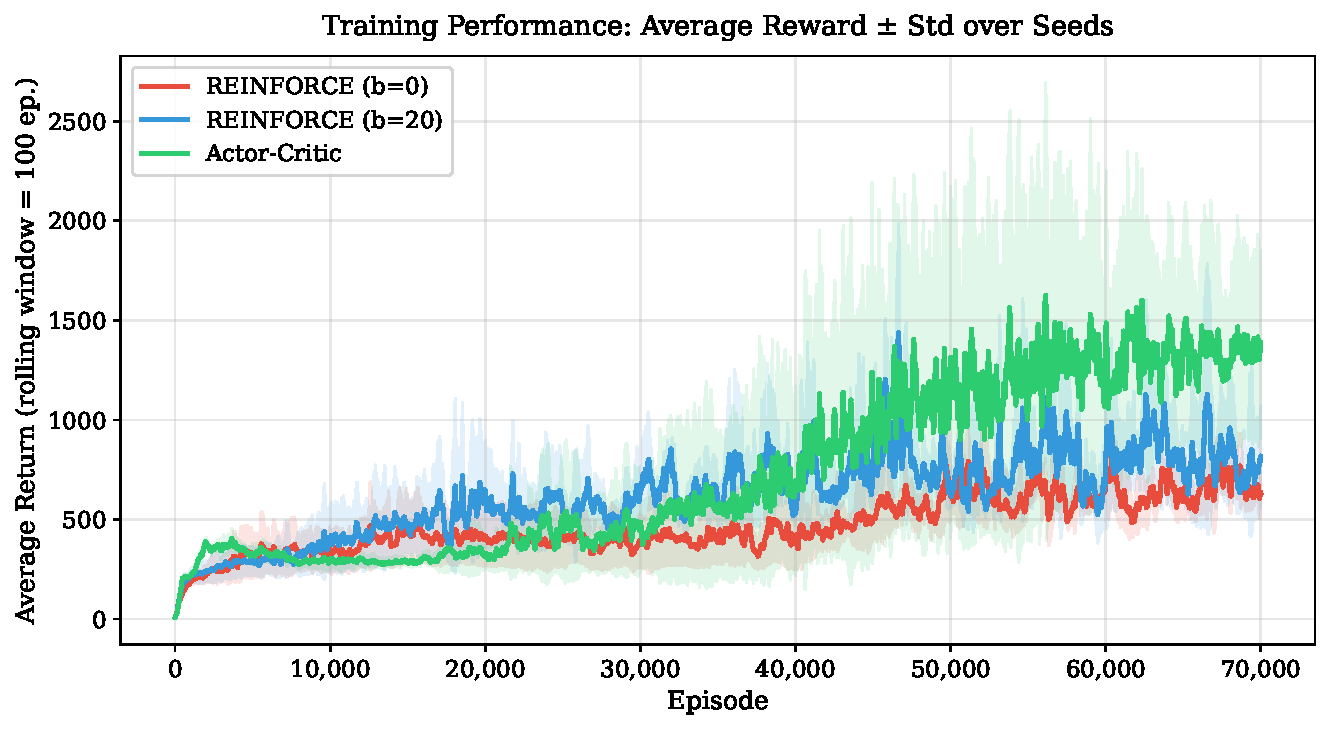
\includegraphics[width=\linewidth]{imgs/experiments_reward.pdf}
    \caption{Average return (rolling window $= 100$ episodes) $\pm$ standard deviation across 3 seeds for REINFORCE ($b{=}0$, $b{=}20$) and Actor-Critic on Hopper-v4.}
    \label{fig:experiments_reward}
\end{figure}

As we can clearly see from Table~\ref{tab:part1_results}, the Actor-Critic achieved the best overall training performance, outperforming the other models 
in terms of highest Best Avg-100 reward (1938), highest Final Avg-100 reward (1360), highest Best Episode reward (3480) and longest average episode length (249 steps).
In turn, REINFORCE with baseline achieved better overall scores than vanilla REINFORCE, improving the Best Avg-100 reward from 1006 to 1807 and the average
episode length from 178 to 215 steps.
Interestingly, despite expecting a gradient-estimator variance reduction with the introduction of a baseline, the opposite behaviour was recorded,
where REINFORCE with baseline exhibited a higher reward standard deviation (399 vs 257) than vanilla REINFORCE.

Figure~\ref{fig:experiments_reward} shows that the Hopper improved its policy throughout training under all algorithms.
However, the Actor-Critic achieved faster policy improvement, reaching larger reward quicker and eventually reaching reward scores that neither of the REINFORCE
variants were able to obtain.

The test results reported in Table~\ref{tab:part1_test_results} support the claim that the Actor-Critic outperformed the other approaches, although substantial variability
across seeds was recorded.
Indeed, the best Actor-Critic seed achieved a mean test return of $3335 \pm 14$ and consistently survived for the full episode ($1000 \pm 0$ steps).
On the other hand, the worst seed achieved a mere $760 \pm 111$ reward score, proving that Actor-Critic did not perform consistenlty across different seeds.
Lower scores but similar variability was observed for both REINFORCE variants.

Overall, the Actor-Critic performed the best both in training and testing among the evaluated methods.
Nevertheless, the large differences between seeds indicate that learning remained sensitive to initialization and stochastic training effects.












\subsection{Part 2 Results: PandaPush Sim-to-Sim Transfer}

Idea:
\begin{itemize}
    \item Show results of each algorithm $\Rightarrow$ SAC + UDR $\rightarrow$ SAC + ADR $\rightarrow$ SAC $\rightarrow$ PPO
    \item Reality gap $\Rightarrow$ vanilla SAC vs upper bound ; SAC + UDR vs upper bound
    \item Mass-sensitivity analysis $\Rightarrow$ vanilla SAC sucks and SAC + UDR achieves better results for general purpose
    \item Again, not sure about the correctness and pretty AI
\end{itemize}

\textbf{(Marco ha messo una tabella in report insights pt2 ma è gigantesca, inserirei separatamente le tabelle per i valori richiesti (Source-Source, Source-Target già fatta))}
\textbf{Risultati PPO per source-source: return -3.485 +- 0.091 sr 20\% +- 0.1, target->target solo su sac}

\begin{table}[h]
\centering
\begin{tabular}{lcc}
\hline
Method & Target Return & Target Success Rate \\ 
\hline
PPO & $-3.496 \pm 0.051$ & $20\% \pm 0.1\%$ \\
SAC (none) & $-0.633 \pm 0.152$ & $97.5\% \pm 0.3\%$ \\
SAC + ADR & $-0.556 \pm 0.044$ & $99.2\%$ \\
\textbf{SAC + UDR} & $\mathbf{-0.509 \pm 0.032}$ & $\mathbf{99.7\%}$ \\
Oracle & $-0.445 \pm 0.019$ & $100\%$ \\
\hline
\end{tabular}
\caption{Target-environment performance comparison.}
\label{table:target_performance}
\end{table}

The results clearly show that SAC outperforms PPO, both on source and training environments \ref{table:target_performance}. Even after an extensive hyperparameter tuning, PPO consistently plateaued around a return of -3.0 and failed to solve the task consistently (success rate:$\sim 20\%$). On the other hand, SAC successfully learned effective pushing policies and transferred well to the target environment.

Uniform Domain Randomization (UDR) achieved the best performance, outperforming both vanilla SAC and Automatic Domain Randomization (ADR). It achieved a target return of -0.509 compared to -0.556 for ADR and -0.633 for vanilla SAC. The policy obtained training directly on the target environment (oracle) achieved the best overall result (-0.445) but is not a valid sim-to-real solution because it has access to target dynamics during training, it only represents the upper bound.

The reality gap can be measured relative to the oracle.
\begin{itemize}
    \item The gap between vanilla SAC and the oracle is $(-0.445)-(-0.633)=0.188$.
    \item The gap between SAC + UDR and the oracle is $(-0.445)-(-0.509)=0.064$.
\end{itemize}

Therefore, the fraction of the gap removed by UDR is
\[
\frac{0.188-0.064}{0.188}=0.6596,
\]
corresponding to approximately 66\%.

This result indicates that UDR eliminates about two-thirds of the performance loss caused by the source-to-target mass shift.

Finally a mass-sensitivity analysis was conducted to further highlight the robustness gained thanks to domain randomization techniques. When evaluated at increasingly heavier masses, vanilla SAC deteriorates from -0.554 at 1 kg to -0.869 at 15 kg. In contrast, UDR only decreases from -0.478 to -0.592 over the same range. This demonstrates that UDR learns a policy that is robust across a wide range of dynamics rather than specialized to a single mass value.

\section{Discussion}

The results highlight how the vanilla REINFORCE algorithm struggled to discover a policy that allows the locomotion of the Hopper, achieving a low average reward during training (around $1006$) and displaying low test returns (ranging from $710$ to $1305$).
Practically this means that the agent cannot effectively hop but at most it stays still trying not to fall and at most leap forward and fall. 

As expected, vanilla REINFORCE struggled due to the high variance of full-trajectory Monte Carlo returns, which causes noisy gradient updates, leading to inefficient learning and slow convergence.

Regarding the time needed for training, this was the fastest among the three with a value of $57.6$ minutes, in fact this is primarily driven by episode length,
the Hopper in this case often falls causing the early termination of the episode (the average episode length is $178$), reducing the computational time needed for the learning process.

Introducing a constant baseline of $b{=}20$ had a positive impact on the agent performance. The peak training average reached $1807$ and the test evaluations showed that the best-performing seed achieved a mean test return of
$2444$.

This means that the agent was able to learn a policy that allowed it to effectively hop and move forward for a longer period of time.
The baseline is subtracted from the Monte Carlo return to reduce the variance of the gradient estimates. This reduces the amount of noise in the gradient updates, leading to a more stable and efficient learning process. 
This also improved the average episode length, which increased from 178 to 215, meaning that the agent was able to stay alive for longer periods of time. 

This is also reflected in the average training time that was significantly higher with a value of $70.3$ minutes, proving that the agent
was not falling for a longer period of time.

While a constant baseline ($b=20$) reduced variance and improved performance over vanilla REINFORCE, it applies a global correction that is identical across all states. Actor-Critic further improved stability by using a state-dependent baseline $V(s)$, which adapts to the local structure of the value function, providing a much more effective variance reduction at each step.

The results obtained in the first part demonstrate that the proposed Actor-Critic framework successfully learned a locomotion policy for the Hopper environment.
Indeed, as Figure~\ref{fig:experiments_reward} shows, the Hopper initially discovered balancing and survival behaviours in the first 40,000 episodes, resulting in relatively
low rewards and short episode lengths.
Subsequently, a sharp performance improvement occurred between 40,000 and 55,000 episodes, corresponding to an increase of both reward
and episode duration, suggesting that the agent discovered forward locomotion for the first time.
After this transition phase, training entered a high-performance regime in which average rewards approached 2000 and individual episodes
occasionally exceeded a reward of 3000.
These results demonstrate that the agent discovered effective hopping.
Nevertheless, training did not fully converge to a stable hopping policy: significant reward variance remained throughout the final stages of training, 
indicating that the learned policy was still too exploratory and stochastic, causing it to be unable to reproduce its best behaviors consistently.

This result represents a substantial improvement compared to earlier Actor-Critic implementations tested during development.
Preliminary versions frequently converged to a "lazy" policy in which the Hopper stood still, which can mathematically occur
due to the Hopper maximizing only the survival component of the reward function.

Standing actions were continuously selected as they tended to achiev high positive advantages, meaning these
actions consistently produced outcomes that were better than the critic’s expectations.
On the other hand, jumping actions continuously turned out to be worse than the critic’s expectations.
This occurred due to the initial usage of the TD(0) target, in which only the immediate subsequent
state was considered, so jumping actions always led to immediate worse states, making them less appealing to a
short-sighted critic and discouraging their exploration.
Therefore, the short-sighted critic reinforced actions that led to immediate better states: standing,
which continued to return a positive reward thanks to the survival component of the reward function, forcing the
Hopper to adopt a reward-exploiting local optimum behavior.

Although such behaviour produced relatively stable trajectories, it prevented the discovery of effective locomotion and resulted in poor returns.
The introduction of GAE, a sigma floor together with advantage normalization, a learned exploration variance, a triggered learning-rate decay mechanism
significantly improved exploration and enabled the policy to free itself from the local optimum, eventually discovering hopping.

The final model's behavioral instability seems to be supported by the critic-loss spikes, which, however, 
should not necessarily be interpreted as training failure.
These spikes are not necessarily indicative of unstable training as reinforcement-learning targets
continuously change together with the current policy, therefore when the actor discovers substantially better trajectories,
previously learned value estimates become obsolete and inaccurate, generating large temporal-difference errors and
consequently large critic-loss spikes. This reasoning proves that the critic loss irregularity is caused by its own outdated
estimates and it trying to keep up with the new updated policy, demonstrating that an unsteady critic loss is quite inevitable
as it is caused by the Reinforcement Learning intrinsic dynamicity.

This interpretation is supported by the fact that critic spikes often coincide with newly discovered high-reward behaviors,
such as the discovery of hopping.

In contrast, actor updates remained remarkably stable throughout training, as advantage normalization successfully bounded
policy updates and prevented gradient explosions despite the highly non-stationary learning process.

Despite these improvements, the final policy still exhibits substantial variability and has not fully converged. Future work
could investigate additional stabilization techniques like TRPO or PPO which exploits trust region and clipped policy
updates (Schulman et al., 2017).

Furthermore, more advanced actor-critic methods for continuous control, such as DDPG and TD3, could be explored,
exploiting double-critic architectures and delayed policy updates, to potentially reduce value-estimation errors
and improve training stability (Fujimoto et al., 2018).


\begin{figure}[htbp]
    \centering
    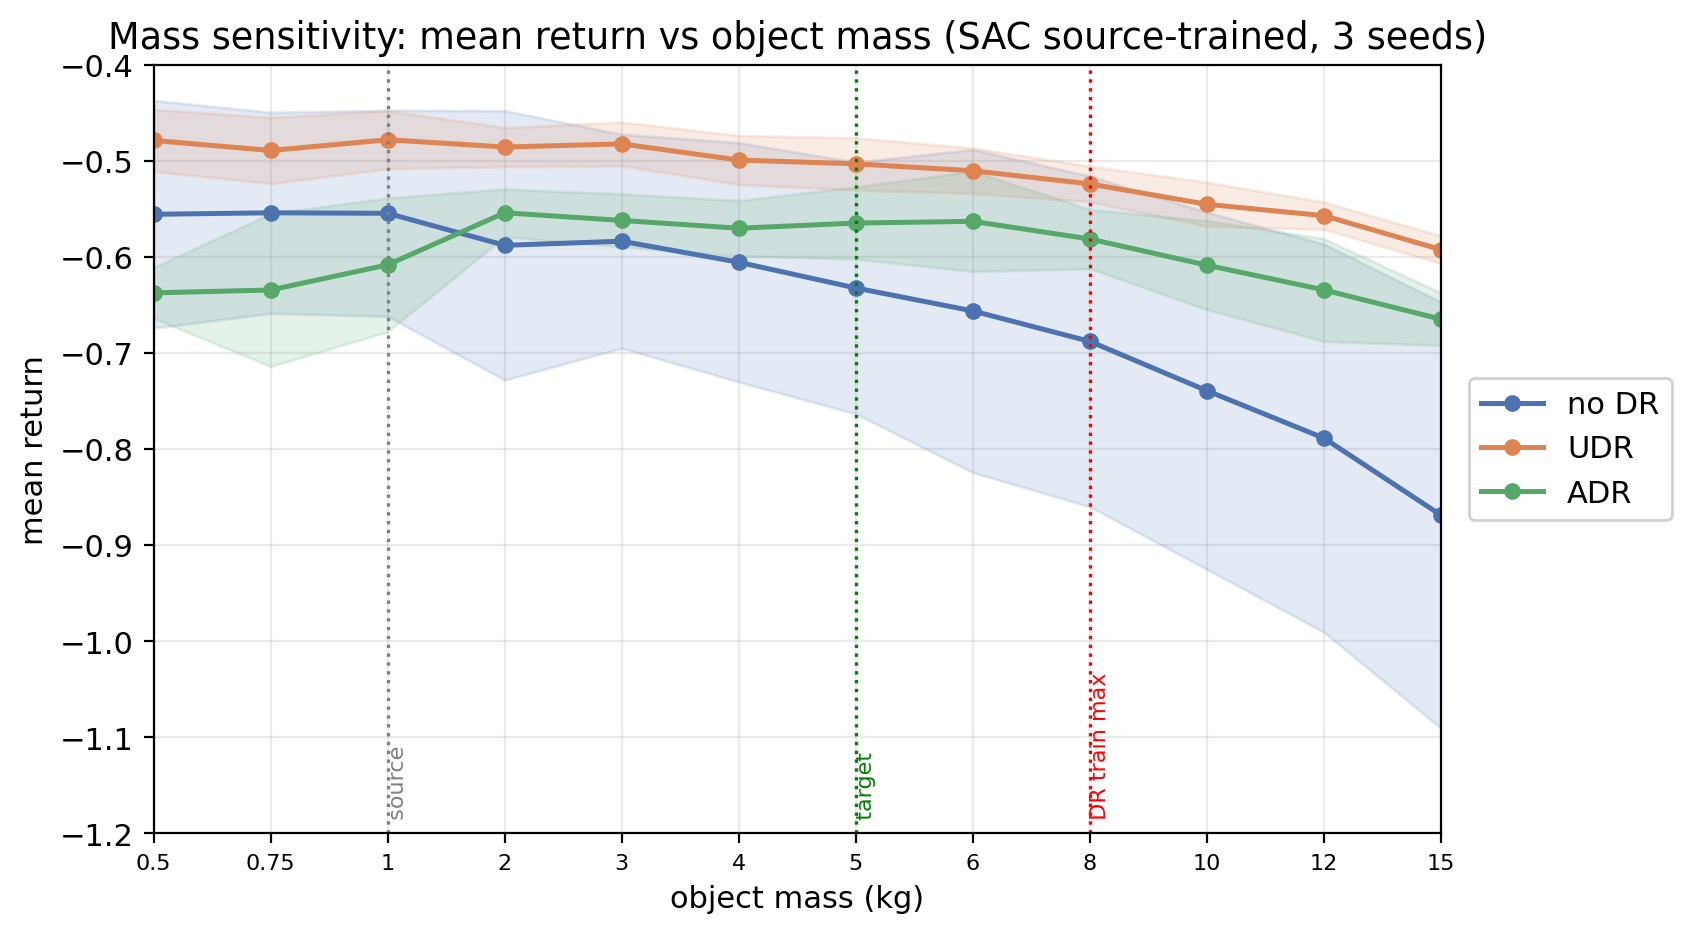
\includegraphics[width=\columnwidth]{imgs/sensitivity_return.png}
    \caption{Mass-sensitivity analysis.}
    \label{fig:sensitivity}
\end{figure}

\section{Conclusion}

This project explored reinforcement learning for continuous control and 
sim-to-real transfer across two tasks. In Part 1, the Actor-Critic algorithm 
equipped with Generalized Advantage Estimation, advantage normalization, 
and learning-rate decay proved to be the strongest performer on the Hopper 
environment, achieving average rewards around 2000 and single episodes 
exceeding 3000, while vanilla REINFORCE and its constant-baseline variant 
served as important stepping stones toward understanding the role of 
variance reduction in policy gradient methods.

In Part 2, the focus shifted to sim-to-real transfer in the PandaPush environment. The experimental results demonstrated
a clear advantage of Soft Actor-Critic (SAC) over Proximal Policy Optimization (PPO), which failed to solve the task within
the available training budget. Among the transfer strategies deployed to fill the reality gap,
Uniform Domain Randomization (UDR) achieved the best overall performance, outperforming both vanilla SAC and
unexpectedly Automatic Domain Randomization (ADR) too.

The final selected approach is therefore SAC combined with UDR. By training on a broad distribution of cube masses,
UDR produced a substantially sturdier policy and reduced the sim-to-real gap by approximately 66\% relative to
the non-randomized baseline. These results confirm the effectiveness of domain randomization as a practical strategy
for improving transfer performance in robotic reinforcement-learning tasks.

\section*{Acknowledgments}

\begin{center}
\begin{minipage}{0.9\columnwidth}

The authors declare that Generative AI tools were not used for writing this project report.

Regarding the development of the submitted project code, the authors declare the use of Generative AI tools as follows:

\begin{itemize}
    \item \textbf{Name and version:} Antigravity IDE with Gemini 3.1 Pro, Gemini 3.5 Flash
    \item \textbf{Publisher:} Google
    \item \textbf{Context and usage:} The tools were used exclusively as coding and research assistants to analyze the literature, 
    produce plot generation scripts, and set up the Weights \& Biases (wandb) framework for logging purposes. 
    All AI-generated suggestions were reviewed and validated by the authors.
\end{itemize}

\end{minipage}
\end{center}



\bibliographystyle{IEEEtran}
\bibliography{sections/bibliography}

\end{document}
